\documentclass[journal,onecolumn,12pt]{IEEEtran}

\usepackage{amsmath}
\usepackage{newtxtext,newtxmath}
\usepackage{graphicx}
\usepackage{tikz}
\usetikzlibrary{arrows.meta,calc,fit,backgrounds}
\usepackage{booktabs}
\usepackage{cleveref}
\usepackage{microtype}
\usepackage[backend=biber,style=ieee,maxbibnames=3,minbibnames=1]{biblatex}
\addbibresource{refs.bib}
\AtEveryBibitem{\clearfield{url}\clearfield{urldate}}
\renewcommand*{\bibfont}{\small}

\begin{document}
\title{Page-Level Handwriting Forgery Detection:\\
Multi-Reference Verification with Calibrated Verdicts}

\author{Lincy~Jenita~J and S.~D.~Lalitha% 
\thanks{The authors are with the Division of Artificial Intelligence and Machine Learning, Karunya Institute of Technology and Sciences, India.}}
\markboth{Page-Level Handwriting Forgery Detection}{Lincy Jenita J and S. D. Lalitha}

\maketitle

\begin{abstract}
\IfFileExists{sections/abstract.tex}{Disputed handwritten scripts, such as an exam answer sheet suspected of being copied in another person's hand, require deciding whether a questioned page is consistent with a writer's earlier pages, yet most deep verifiers compare single words or signatures. We study page-level, multi-reference verification: a full page is embedded as an attention-pooled bag of ink patches by a ResNet-18 trained from scratch with content-matched hard negatives and distillation from a frozen DINOv2 teacher, and one or several reference pages are fused into a calibrated three-way verdict (consistent, inconclusive, likely forged). We train three seeds on IAM and CVL with writer-disjoint splits and test exactly once on held-out writers and on Firemaker, a separate corpus never used for training or tuning. The model reaches 2.35\% EER on IAM and 7.30\% on CVL, against 5.44\% and 15.02\% for frozen DINOv2 features, 11.1\% and 23.1\% for HOG, and 23.2\% and 30.6\% for an untrained network. On Firemaker, ordinary writing transfers across corpora (3.3\% EER), but upper-case copying (23.9\%) and deliberately disguised writing (32.0\%) break it. On one fixed set of writers, three reference pages lower the centroid-fusion EER from 2.25\% to 1.22\% on IAM and from 6.76\% to 5.19\% on CVL, and the maximum rule alone reaches 3.31\% on CVL, a post-hoc observation. A verdict calibrated on validation data leaves 8.5\% of CVL trials inconclusive and is wrong on 2.8\% of the rest. No ablated training ingredient shows a clear benefit in a short, single-seed, 40-epoch comparison. No public data show one person imitating another, so these are not forgery detection rates, and the font-rendered pages we tested say nothing about learned imitation.
}{}
\end{abstract}

\begin{IEEEkeywords}
handwriting verification, forgery detection, writer verification, metric learning, knowledge distillation, calibration
\end{IEEEkeywords}

\section{Introduction}
Handwritten examination scripts, wills, contracts and notes are routinely disputed.
A typical case is an answer sheet whose ownership is questioned because another person is suspected of copying the answers in an imitation of the owner's handwriting.
The owner can then offer earlier genuine scripts as references, and an examiner must decide whether the questioned script is consistent with them.
This is a \emph{page-level, multi-reference} verification problem: the evidence is a complete script, not a single word, sentence or signature, and several known pages are available.

Most deep-learning work on handwriting is organised differently.
Writer identification and retrieval systems assign a page to one of many known writers or rank a collection by similarity~\cite{xing2016deepwriter,he2020fragnet,christlein2017unsupervised,raven2024selfsupervised,peer2023towards}.
Verification work compares a pair of samples, usually words, text patches or signatures~\cite{adak2019intravariable,shaikh2020attention,dey2017signet,chauhan2024selfsupervised}.
Little of it combines a whole questioned page with several reference pages, reports a calibrated degree of support, or allows the system to answer ``inconclusive''.

A further difficulty is the threat model.
Public datasets contain genuine pages by many writers, but almost none contain a person deliberately imitating another.
At the same time, generative models can now imitate a given writing style~\cite{nikolaidou2023wordstylist,nikolaidou2024diffusionpen,vanherle2024vatr,mayr2024zeroshot}.

This paper builds and evaluates a page-level verifier under these conditions.
Our contributions are:
\begin{itemize}
\item A page-level verifier that embeds a full script as an attention-pooled bag of ink patches and compares a questioned page with one or several reference pages, with four fusion rules evaluated.
\item Content-matched hard negatives on CVL (different writers copying the same text), a calibrated three-way verdict with thresholds fixed on validation data, and a compact ResNet-18 student distilled from a frozen self-supervised ViT; an ablation shows no clear benefit of any single ingredient in a short schedule.
\item An evaluation protocol with writer-disjoint splits, a cross-dataset test on a corpus never used for training or tuning, a controlled multi-reference study, and explicit reporting of what the available data cannot show, including that deliberate style change breaks the model.
\end{itemize}
To our knowledge, no prior writer-verification work combines these elements, but we do not claim that any single component is new.
Distillation and likelihood-ratio reporting each have precedent~\cite{tsourounis2023leveraging,ypma2024evidential}.

We study four research questions.
\textbf{RQ1:} how well does a page-level model separate writers, and does it beat untrained and frozen-feature baselines?
\textbf{RQ2:} does adding reference pages help, and which fusion rule is best?
\textbf{RQ3:} does the model transfer to a corpus recorded with a different scanner and protocol (Firemaker), including pages written in a disguised style?
\textbf{RQ4:} which training ingredients matter: distillation, attention pooling, content-matched batches, writer mining, patch count and augmentation?

\section{Related Work}
\textbf{Writer identification and retrieval.}
Text-independent writer identification with CNNs was established by DeepWriter~\cite{xing2016deepwriter}, and later work introduced fragment-based and attention-based models~\cite{he2020fragnet,kumar2024attention}.
Unsupervised and self-supervised representations have become competitive for retrieval on historical and modern pages~\cite{christlein2017unsupervised,peer2023towards,raven2024selfsupervised,maitra2024decorrelationbased}.
Recent studies analyse which pipeline factors matter for historical writer identification~\cite{rasyidi2025beyond}.
These systems answer ``which writer'' or ``which pages are similar''; they do not output a verification decision for a claimed writer.

\textbf{Handwriting verification.}
Adak et al.\ study writer identification and verification from intra-writer variation~\cite{adak2017an,adak2019intravariable}.
Shaikh et al.\ propose an attention-based writer-independent verifier~\cite{shaikh2020attention}, and self-supervised pre-training has been applied to the same task~\cite{chauhan2024selfsupervised,wang2023csslrha}.
Signature verification uses twin networks and metric learning~\cite{dey2017signet,huang2023multiscale,parracho2025signature}.
Our setting differs in using complete pages and several references.

\textbf{Generated handwriting as a threat.}
Diffusion and transformer generators produce handwriting in a target style from short style samples~\cite{nikolaidou2023wordstylist,nikolaidou2024diffusionpen,vanherle2024vatr}, including paragraphs~\cite{mayr2024zeroshot}.
Synthetic data has also been used to pre-train handwriting models~\cite{pippi2023evaluating}.

\textbf{Distillation, fusion and calibration.}
Knowledge distillation~\cite{hinton2015distilling} has been used in offline signature verification~\cite{tsourounis2023leveraging}.
Self-supervised ViTs such as DINOv2~\cite{oquab2023dinov} provide strong frozen features.
Forensic work argues that the strength of evidence should be expressed as a likelihood ratio~\cite{ypma2024evidential}, and modern networks are often poorly calibrated~\cite{guo2017on}.
We adopt these ideas for page-level handwriting verification.

\section{Data}
\label{sec:data}
We use three corpora, all English.
The IAM database~\cite{marti2002iam} provides forms by 657 writers; the CVL database~\cite{kleber2013cvl} provides pages by 310 writers who copy the same texts, of which we use the English texts only (the German excerpt is excluded); and Firemaker~\cite{bulacu2003firemaker} provides four pages for each of 250 writers.
Splits are writer-disjoint (seed 42); writer identifiers are prefixed by corpus.
Firemaker is never used for training, validation or threshold selection and serves as a cross-dataset test.
Its third page is written in a deliberately changed style, i.e.\ self-disguise rather than imitation of another person, so we report it as a stress test of intra-writer variation and not as forgery.
\Cref{tab:data} lists the sizes after preprocessing, generated from the manifest.

\begin{table}[t]
\caption{Writers and pages after preprocessing. IAM writers with a single page contribute two half-page views to training only; Firemaker is used for testing only.}
\label{tab:data}
\centering\scriptsize
\setlength{\tabcolsep}{3pt}
\resizebox{\columnwidth}{!}{\begin{tabular}{lrrrrrr}
\toprule
& \multicolumn{2}{c}{Train} & \multicolumn{2}{c}{Validation} & \multicolumn{2}{c}{Test} \\
Corpus & Writers & Pages & Writers & Pages & Writers & Pages \\
\midrule
IAM & 507 & 1262 & 50 & 190 & 99 & 392 \\
CVL (English) & 217 & 909 & 31 & 127 & 62 & 254 \\
Firemaker & -- & -- & -- & -- & 250 & 1000 \\
\bottomrule
\end{tabular}
}
\end{table}


\section{Method}
\begin{figure*}[t]
\centering
\resizebox{\textwidth}{!}{% Architecture figure (TikZ). \input inside figure*; needs tikz libraries: positioning, arrows.meta, calc, fit, backgrounds.
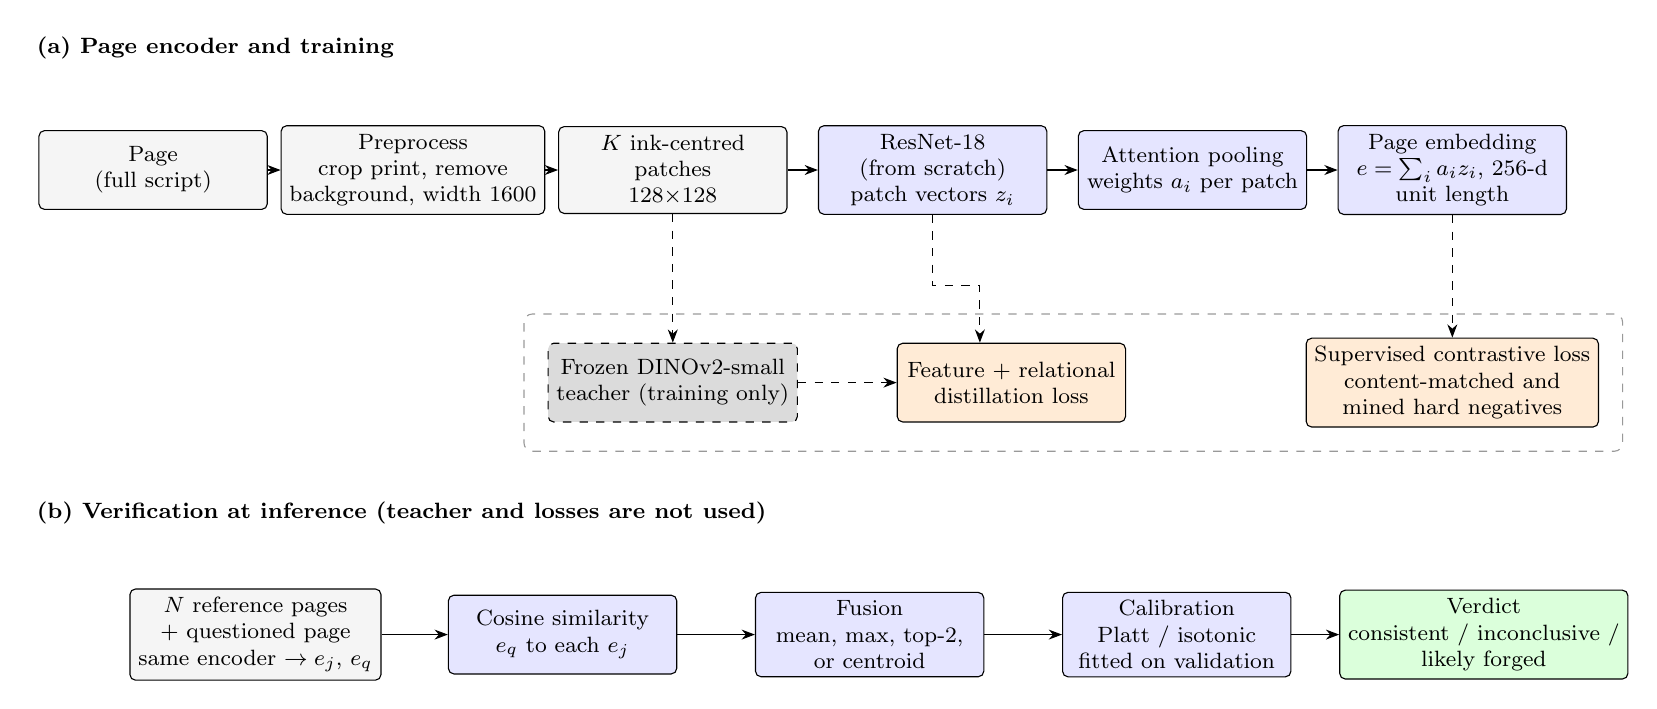
\begin{tikzpicture}[
  font=\footnotesize, >=Stealth,
  box/.style={draw, rounded corners=2pt, minimum height=10mm, minimum width=29mm, align=center, fill=gray!8, inner sep=3pt},
  netbox/.style={box, fill=blue!10},
  lossbox/.style={box, fill=orange!16},
  frozenbox/.style={box, fill=gray!28, dashed},
  outbox/.style={box, fill=green!14},
  panel/.style={font=\footnotesize\bfseries, anchor=west}
]
% ================= (a) embedding network and training =================
\node[panel] at (-1.6,1.55) {(a) Page encoder and training};
\node[box]    (page)  at (0,0)    {Page\\(full script)};
\node[box]    (pre)   at (3.3,0) {Preprocess\\crop print, remove\\background, width 1600};
\node[box]    (patch) at (6.6,0)  {$K$ ink-centred\\patches\\$128{\times}128$};
\node[netbox] (cnn)   at (9.9,0) {ResNet-18\\(from scratch)\\patch vectors $z_i$};
\node[netbox] (att)   at (13.2,0) {Attention pooling\\weights $a_i$ per patch};
\node[netbox] (emb)   at (16.5,0){Page embedding\\$e=\sum_i a_i z_i$, 256-d\\unit length};
\draw[->] (page) -- (pre);  \draw[->] (pre) -- (patch);  \draw[->] (patch) -- (cnn);
\draw[->] (cnn) -- (att);   \draw[->] (att) -- (emb);

\node[frozenbox] (teach) at (6.6,-2.7)  {Frozen DINOv2-small\\teacher (training only)};
\node[lossbox]   (dist)  at (10.9,-2.7) {Feature + relational\\distillation loss};
\node[lossbox]   (sup)   at (16.5,-2.7){Supervised contrastive loss\\content-matched and\\mined hard negatives};
\draw[->, dashed] (patch.south) -- (teach.north);
\draw[->, dashed] (teach.east) -- (dist.west);
\draw[->, dashed] (cnn.south) -- ++(0,-0.9) -| ([xshift=-4mm]dist.north);
\draw[->, dashed] (emb.south) -- (sup.north);

% ================= (b) verification at inference =================
\node[panel] at (-1.6,-4.35) {(b) Verification at inference (teacher and losses are not used)};
\node[box]    (refs) at (1.3,-5.9)  {$N$ reference pages\\+ questioned page\\same encoder $\to e_j,\,e_q$};
\node[netbox] (cos)  at (5.2,-5.9)  {Cosine similarity\\$e_q$ to each $e_j$};
\node[netbox] (fuse) at (9.1,-5.9)  {Fusion\\mean, max, top-2,\\or centroid};
\node[netbox] (cal)  at (13.0,-5.9) {Calibration\\Platt / isotonic\\fitted on validation};
\node[outbox] (verd) at (16.9,-5.9) {Verdict\\consistent / inconclusive /\\likely forged};
\draw[->] (refs) -- (cos);
\draw[->] (cos) -- (fuse); \draw[->] (fuse) -- (cal); \draw[->] (cal) -- (verd);

\begin{scope}[on background layer]
  \node[draw=black!40, dashed, rounded corners=3pt, fit=(teach)(dist)(sup), inner sep=3mm] {};
\end{scope}
\end{tikzpicture}
}
\caption{Overview. (a) Each page is cut into ink-centred patches, encoded by a ResNet-18 trained from scratch and pooled by attention into one page embedding; a frozen DINOv2 teacher is used only during training. (b) At inference the questioned page is compared with $N$ reference pages, the scores are fused and calibrated, and a three-way verdict is returned.}
\label{fig:arch}
\end{figure*}

\subsection{Problem and notation}
Given a claimed writer with $N\ge1$ reference pages $R=\{r_1,\dots,r_N\}$ and one questioned page $q$, the system returns a similarity score $s(q,R)$ and a verdict.
All pages are embedded by one network $f$ into unit vectors, so that $s$ is a function of cosine similarities.

\subsection{Preprocessing}
Each page is converted to gray scale and the printed parts of the forms are removed: for IAM the printed header and footer are cropped using long horizontal separator lines, and for CVL the printed source text above the first separator is cropped.
The paper tone and scanner shading are removed by dividing by a smoothed morphological-closing background estimate.
Pages are resized to a width of 1600 px, which keeps stroke scale comparable across 300~dpi scans.
Pages with an ink fraction below $0.25\%$ are discarded as blank, and duplicate pages are removed by hash.

\subsection{Page encoder}
A page is treated as a bag of $K$ patches of $128\times128$ pixels.
Patches are centred on randomly chosen ink pixels and kept only if their ink fraction passes a threshold; the threshold is lowered progressively (5\%, 3\%, 1.5\%, 0.8\%) when a page has too few dense windows, and a page with no usable ink is rejected instead of being padded.
A ResNet-18~\cite{he2015deep} with a one-channel stem, randomly initialised, maps each patch to a 256-dimensional vector $z_i$.
Attention pooling~\cite{ilse2018attentionbased} computes weights $a_i=\mathrm{softmax}_i\big(w^\top\tanh(Vz_i)\big)$ and the page embedding $e=\mathrm{normalise}\big(\sum_i a_i z_i\big)$.
Training uses $K=16$ random patches per page with augmentation (rotation $\pm3^\circ$, scale $\pm10\%$, contrast and brightness, blur, noise and JPEG artefacts); evaluation uses $K=64$ deterministic patches per page, chosen by a seed derived from the page path.

\subsection{Training objective}
The main loss is the supervised contrastive loss~\cite{khosla2020supervised} with temperature $\tau=0.1$ on page embeddings.
Each batch contains $W=12$ writers with two different pages each.
Two kinds of batch are mixed.
\emph{IAM batches} use random writers and two pages of each writer (or the top and bottom halves of the handwriting area for writers with a single page).
\emph{Content-matched CVL batches} (40\% of steps) choose two texts and use only writers who wrote both; hence all negatives in the batch share text with the positives' texts, while the two pages of a positive pair differ in text.
In addition, every 10 epochs the writer centroids are computed with the EMA model and, with probability $0.5$, a batch is built from a writer and its nearest neighbours (hard-writer mining).

\subsection{Distillation from a frozen teacher}
A frozen DINOv2-small~\cite{oquab2023dinov} teacher embeds the same augmented patches (resized to $126\times126$).
Two auxiliary losses transfer its structure to the student.
The feature term is $1-\cos\big(g(z_i),t_i\big)$ with a linear head $g$ and teacher embedding $t_i$.
The relational term is $\mathrm{KL}\big(\mathrm{softmax}(S^{T}_{i\cdot}/\tau)\,\|\,\mathrm{softmax}(S^{S}_{i\cdot}/\tau)\big)$ between the patch-to-patch cosine similarity matrices of teacher and student, applied to patches and to page embeddings.
The total loss is $\mathcal{L}_{\mathrm{SupCon}}+0.5\,\mathcal{L}_{\mathrm{feat}}+0.5\,\mathcal{L}_{\mathrm{rel}}$.
The teacher is not used at inference; the deployed model is the student alone.

\subsection{Multi-reference scoring, calibration and verdict}
For $N$ references we compare four fusion rules: the mean cosine, the maximum cosine, the mean of the two largest cosines, and the cosine to the renormalised centroid of the reference embeddings.
Scores are calibrated by logistic (Platt) regression and isotonic regression fitted on validation trials only.
The verdict uses two thresholds fixed on validation data: a page is \emph{consistent} if $s\ge\tau_{\mathrm{hi}}$, the 99th percentile of validation impostor scores; \emph{likely forged} if $s\le\tau_{\mathrm{lo}}$, the 1st percentile of validation genuine scores; and \emph{inconclusive} otherwise.
Attention weights give a patch-level map of which regions drove the score.

\section{Experimental Setup}
\label{sec:exp}
\subsection{Implementation}
The student is trained from scratch with AdamW (learning rate $3\times10^{-4}$, weight decay $10^{-4}$), a 5-epoch warm-up and cosine decay over 120 epochs, mixed precision, gradient clipping at 1.0, and an exponential moving average of weights (decay 0.999) that is used for validation and testing.
Model selection uses the mean of the IAM and CVL validation equal error rates, and training stops after 30 epochs without improvement.
Experiments ran on a single laptop GPU (RTX 4050, 6~GB) in a Docker container based on PyTorch 2.6 with CUDA 12.4.
Main results are the mean and standard deviation over three seeds.

\subsection{Protocol and metrics}
For single-reference evaluation every pair of pages from the same dataset and split is scored; same-writer pairs are genuine and different-writer pairs are impostors, so impostor pairs on CVL include pairs that copy the same text.
For multi-reference evaluation we draw 1000 genuine and 1000 impostor trials per setting with $N\in\{1,2,3,5\}$ references.
We report the equal error rate (EER), the area under the ROC curve (AUC), and the false accept rate at a 1\% and 10\% false reject rate.
Confidence intervals are 95\% bootstrap intervals over writers.
Thresholds and calibrators are fitted on validation data and applied unchanged to the test sets.

\subsection{Baselines}
We compare with (i) a randomly initialised encoder, (ii) the same encoder with batch-normalisation statistics adapted on the data but no label training, (iii) frozen DINOv2-small features averaged over patches, and (iv) HOG features averaged over patches.

\IfFileExists{sections/results.tex}{\section{Results}
\label{sec:results}
All numbers are test results, in percent, as mean $\pm$ standard deviation over three seeds, unless stated.
The three seeds share the same writer-disjoint splits.

\subsection{RQ1: separating writers}
\Cref{tab:main} compares our model with the baselines.
On held-out writers the student reaches an EER of $2.35\pm0.12$ on IAM and $7.30\pm0.29$ on CVL (AUC 0.996 and 0.968).
Frozen DINOv2-small features, the teacher without any training on handwriting, give 5.44 and 15.02, so the student halves the error of the teacher on both corpora; HOG and an untrained CNN are far behind.
The 95\% bootstrap intervals over writers are wide (1.7 to 4.2 on IAM, 4.7 to 12.0 on CVL, per seed) because only 99 and 62 writers are available.
Test error is higher than validation error (IAM $0.90\pm0.31$, CVL $5.81\pm0.15$), which shows how optimistic the validation numbers were.
At a strict operating point the picture is weaker: with the false reject rate fixed at 1\%, the false accept rate is $10.1\pm1.2\%$ on IAM and $80.2\pm12.4\%$ on CVL, and at 10\% it is 0 and $3.5\pm0.4\%$.
The content-matched CVL pairs are therefore the hard case, and a single page pair is not enough evidence for a high-stakes decision.
On validation, an untrained encoder with batch-normalisation statistics adapted to the data already reaches 8.5\% on IAM and 21.3\% on CVL, which suggests that corpus-level cues such as scanner and paper carry part of the IAM signal.

\begin{table}[t]
\caption{Single-reference test results over all page pairs. The untrained CNN is averaged over three seeds; HOG and frozen DINOv2 have no training and are deterministic.}
\label{tab:main}
\centering\scriptsize
\setlength{\tabcolsep}{3pt}
\resizebox{\columnwidth}{!}{\begin{tabular}{lcccc}
\toprule
& \multicolumn{2}{c}{IAM} & \multicolumn{2}{c}{CVL} \\
Model & EER & AUC & EER & AUC \\
\midrule
Random CNN & 22.27$\pm$0.22 & 0.873$\pm$0.002 & 34.33$\pm$0.40 & 0.734$\pm$0.001 \\
HOG & 14.10 & 0.949 & 23.59 & 0.839 \\
DINOv2-small (frozen) & 5.03 & 0.992 & 16.00 & 0.911 \\
\midrule
Ours, 1 seed(s) & \textbf{0.48} & \textbf{1.000} & \textbf{5.90} & \textbf{0.984} \\
\bottomrule
\end{tabular}
}
\end{table}

\Cref{fig:train} shows validation EER and loss for the three seeds; after the best epoch the validation EER plateaus and fluctuates between about 3.5\% and 4.3\%, so the selected checkpoint is chosen from a noisy plateau.
The per-seed results (\Cref{tab:seeds}) differ by at most 0.3 EER on IAM and 0.7 on CVL, so the reported means are stable across seeds.

\begin{figure*}[t]
\centering
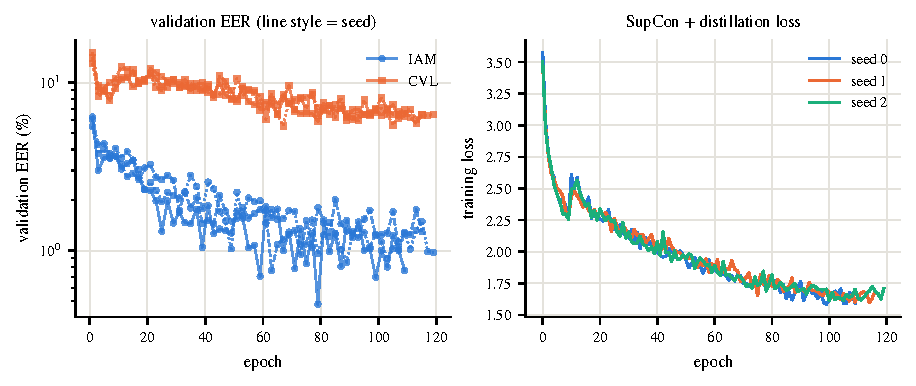
\includegraphics[width=\textwidth]{figures/fig_training_curves}
\caption{Validation EER (left, log scale; line style = seed) and training loss (right) of the three main runs.}
\label{fig:train}
\end{figure*}

\begin{table}[t]
\caption{Per-seed test results (EER, \%) and the share of inconclusive CVL verdicts.}
\label{tab:seeds}
\centering\scriptsize
\setlength{\tabcolsep}{2.5pt}
\resizebox{\columnwidth}{!}{\begin{tabular}{lccccc}
\toprule
Seed & IAM EER & CVL EER & Firemaker p4 & Firemaker p3 & CVL inconcl. (\%) \\
\midrule
0 & 2.20 & 7.16 & 3.00 & 31.40 & 7.8 \\
1 & 2.50 & 7.71 & 3.40 & 31.80 & 8.8 \\
2 & 2.36 & 7.04 & 3.60 & 32.80 & 8.9 \\
\bottomrule
\end{tabular}
}
\end{table}

\subsection{RQ2: more reference pages and fusion rules}
\Cref{fig:multiref} evaluates $N=1,2,3$ references on one fixed set of writers (45 on IAM, 62 on CVL, the writers with at least four pages), so that the writer set does not change with $N$.
With the centroid rule, the one used for calibration, EER falls from $2.25\pm0.05$ to $1.57\pm0.11$ and $1.22\pm0.12$ on IAM, and from $6.76\pm0.38$ to $5.22\pm0.54$ and $5.19\pm0.73$ on CVL.
On the 17 IAM writers with at least six pages, five references give $0.81\pm0.22$ against $1.96\pm0.31$ for one; CVL has too few such writers (three) for $N=5$.
The fusion rule matters.
On CVL the maximum of the cosine similarities is best at $N=3$ ($3.31\pm0.20$, against $5.99\pm0.71$ for the mean and $5.13\pm0.18$ for the two largest), while on IAM the centroid is best at three references and the maximum at two.
The centroid was fixed on validation, where it was best; that the maximum is better on test CVL is a post-hoc observation that we have not confirmed on separate data.
The seed-0 bootstrap intervals for $N=1$ and $N=3$ overlap (CVL centroid 3.6 to 10.8 and 2.3 to 9.0), so the gain from extra references is consistent in direction but not established for the population of writers.

\begin{figure*}[t]
\centering
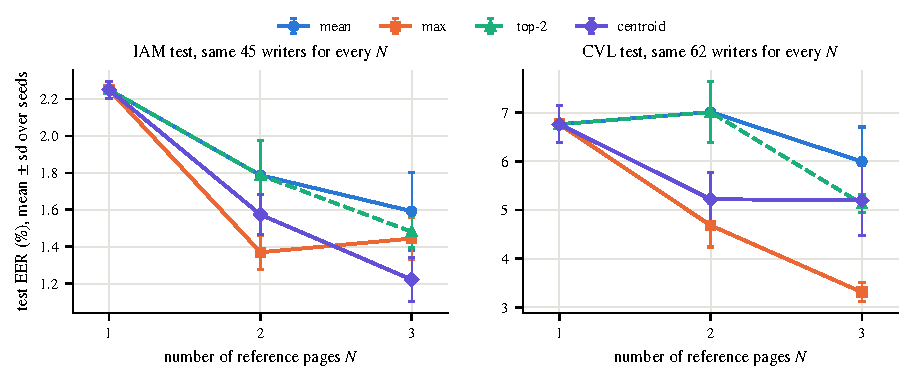
\includegraphics[width=\textwidth]{figures/fig_multiref_test}
\caption{Test EER against the number of reference pages for the four fusion rules, on one fixed set of writers for every $N$ (mean $\pm$ sd over three seeds). More references help, and the maximum rule is best on CVL.}
\label{fig:multiref}
\end{figure*}

\subsection{RQ3: cross-corpus transfer and disguise}
\Cref{tab:fm} and \Cref{fig:fm} use Firemaker, which differs in scanner and protocol and was never used for training, validation or thresholds.
For ordinary writing (page 1 against the self-written page 4) the EER is $3.33\pm0.25$ (AUC 0.994), close to IAM, so the representation transfers.
It does not survive a deliberate change of writing.
Upper-case copying raises the EER to $23.87\pm0.47$ and the disguised page to $32.00\pm0.59$.
The mean same-writer cosine falls from 0.978 to 0.906 and 0.874, while the mean other-writer cosine stays at about 0.79: disguise moves genuine pairs towards impostors.
A writer who simply changes style can therefore be rejected by the system, and the same effect would help a forger who copies a style.

\begin{table}[t]
\caption{Firemaker (250 writers): page 1 against pages 4, 2 and 3 of the same writers.}
\label{tab:fm}
\centering\scriptsize
\setlength{\tabcolsep}{2.5pt}
\resizebox{\columnwidth}{!}{\begin{tabular}{lcccc}
\toprule
Pair (same writer) & EER & AUC & Same-writer cos. & Other-writer cos. \\
\midrule
p1 vs p4 (natural, self-written) & 3.33$\pm$0.25 & 0.994$\pm$0.000 & 0.978$\pm$0.004 & 0.790$\pm$0.031 \\
p1 vs p2 (upper case) & 23.87$\pm$0.47 & 0.847$\pm$0.005 & 0.906$\pm$0.013 & 0.791$\pm$0.029 \\
p1 vs p3 (disguised) & 32.00$\pm$0.59 & 0.747$\pm$0.012 & 0.874$\pm$0.017 & 0.791$\pm$0.030 \\
\bottomrule
\end{tabular}
}
\end{table}

\begin{figure}[t]
\centering
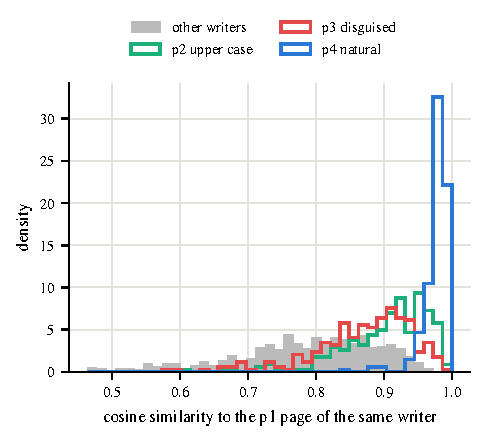
\includegraphics[width=\columnwidth]{figures/fig_firemaker}
\caption{Cosine similarity to the page 1 of the same writer on Firemaker (seed 0). Natural writing is clearly separated from other writers; disguise and upper case overlap them.}
\label{fig:fm}
\end{figure}

\subsection{RQ4: training ingredients}
\Cref{tab:abl} lists validation EER for six variants against the full model, all trained for 40 epochs with one seed.
No ingredient shows a clear benefit.
Removing distillation (4.38 against 5.35 mean EER), content-matched batches (4.57) or augmentation (4.88) gives a lower error than the full model, and mean pooling, no mining and eight patches (5.29, 5.25, 5.15) are within 0.2 of it.
The seed-to-seed spread of the main runs is about 0.2 in mean validation EER (3.19, 3.57 and 3.31), so only differences above that deserve attention, and with one seed per variant we cannot tell whether the lower values of the three variants are real.
What we can say is that, in this short schedule, none of the five training ingredients is demonstrated to help; the 120-epoch main model (mean validation EER 3.19 to 3.57) is better than every 40-epoch variant, which suggests that training length matters more than any single ingredient, although the two schedules also differ in warm-up and patience.

\begin{table}[t]
\caption{Ablations on validation (EER, \%; 40 epochs, one seed). The 120-epoch main model reaches a mean of 3.19 to 3.57 over three seeds.}
\label{tab:abl}
\centering\scriptsize
\setlength{\tabcolsep}{3pt}
\resizebox{\columnwidth}{!}{\begin{tabular}{lccc}
\toprule
Variant & IAM EER & CVL EER & Mean \\
\midrule
Full model (40 epochs) & 1.72 & 8.98 & 5.35 \\
No distillation & 1.22 & 7.53 & 4.38 \\
Mean pooling & 2.47 & 8.10 & 5.29 \\
No content-matched batches & 1.71 & 7.42 & 4.57 \\
No writer mining & 2.05 & 8.45 & 5.25 \\
8 patches per page & 2.53 & 7.77 & 5.15 \\
No augmentation & 1.74 & 8.02 & 4.88 \\
\bottomrule
\end{tabular}
}
\end{table}

\subsection{Calibrated verdicts}
Raw cosine scores are not probabilities: their expected calibration error is 0.22 on both corpora.
Platt scaling reduces it to 0.070 and 0.076, and isotonic regression to 0.009 and 0.020, all fitted on validation only.
\Cref{tab:verdict} gives the three-way verdict for three references.
On CVL, 8.5\% of trials are inconclusive; of the 91.5\% that are decided, 2.8\% are wrong.
IAM is separable on validation, so the 99th percentile of impostor scores lies below the 1st percentile of genuine scores; we then use one threshold and no inconclusive band (error 0.7\%), and the IAM verdict should not be read as evidence that the problem is easy (\Cref{sec:discussion}).

\begin{table}[t]
\caption{Three-way verdict on test trials with three references (centroid rule), thresholds from validation only.}
\label{tab:verdict}
\centering\scriptsize
\setlength{\tabcolsep}{2.5pt}
\resizebox{\columnwidth}{!}{\begin{tabular}{lccccc}
\toprule
Corpus & Consistent & Likely forged & Inconclusive & Error (decided) & ECE (Platt) \\
\midrule
IAM & 49.7$\pm$0.2 & 50.3$\pm$0.2 & 0.0$\pm$0.0 & 0.68$\pm$0.13 & 0.070$\pm$0.006 \\
CVL & 47.8$\pm$0.8 & 43.7$\pm$1.3 & 8.5$\pm$0.5 & 2.82$\pm$0.21 & 0.076$\pm$0.011 \\
\bottomrule
\end{tabular}
}
\end{table}

\begin{figure}[t]
\centering
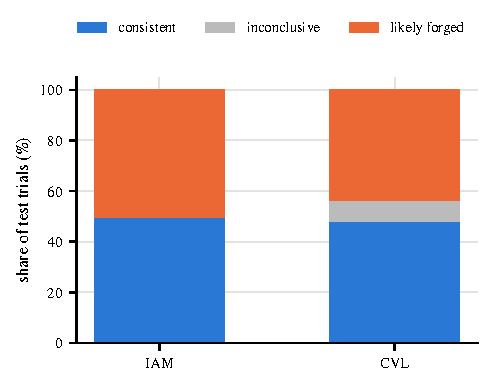
\includegraphics[width=\columnwidth]{figures/fig_verdict}
\caption{Share of test trials judged consistent, inconclusive and likely forged (mean over three seeds, three references).}
\label{fig:verdict}
\end{figure}

\begin{figure*}[t]
\centering
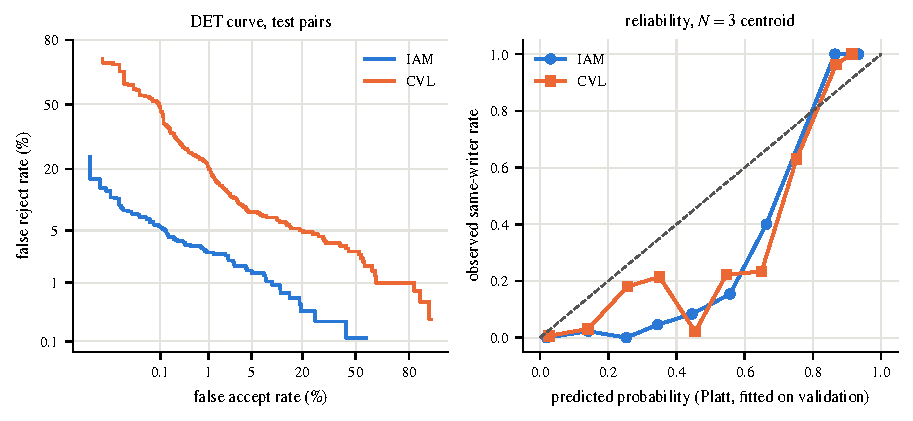
\includegraphics[width=\textwidth]{figures/fig_det_calibration}
\caption{Left: DET curves on test page pairs. Right: reliability of the Platt-calibrated probability for three references (calibrator fitted on validation); the Platt sigmoid is over-confident in the middle range (for example, predicted 0.66 against observed 0.40 on IAM) and under-confident at the top, which is why isotonic regression has the lower ECE.}
\label{fig:det}
\end{figure*}

\subsection{Synthetic pages}
\Cref{tab:syn} tests the 1362 font-rendered pages of the Kaggle set (and 990 real pages by unknown writers as a control) against every real test page, using the validation threshold at the 99th percentile of impostor scores.
Font renderings are accepted for 0.03\% of page pairs on IAM and for none on CVL, but unrelated real pages are accepted at a similar rate, and all score far below same-writer pairs.
Per page, 5.0\% of font pages (IAM threshold) are accepted by at least one of the 99 test writers, against 17.2\% of the real control pages.
The test therefore shows that fonts are not mistaken for real writers in this scan domain; it says nothing about learned imitation.

\begin{table}[t]
\caption{Kaggle pages scored against real test pages (single reference, validation threshold).}
\label{tab:syn}
\centering\scriptsize
\setlength{\tabcolsep}{2.5pt}
\resizebox{\columnwidth}{!}{\begin{tabular}{llccc}
\toprule
Corpus & Kaggle pages & Pairs accepted (\%) & Mean cosine & Pages accepted by $\geq$1 writer (\%) \\
\midrule
IAM & font-rendered & 0.033$\pm$0.023 & 0.47$\pm$0.01 & 5.0$\pm$2.3 \\
IAM & real, unknown writer & 0.144$\pm$0.035 & 0.52$\pm$0.00 & 17.2$\pm$4.9 \\
CVL & font-rendered & 0.000$\pm$0.000 & 0.39$\pm$0.02 & 0.0$\pm$0.0 \\
CVL & real, unknown writer & 0.003$\pm$0.003 & 0.48$\pm$0.02 & 0.4$\pm$0.2 \\
\bottomrule
\end{tabular}
}
\end{table}

\subsection{Where the model looks}
\Cref{fig:att} shows attention maps for four validation pages.
Removing the 25\% most attended patches lowers the cosine to a same-writer reference by 0.0043 on average, against 0.0022 for random patches (60 validation pairs, pair-to-pair standard deviation about 0.04).
The difference is too small to call the maps an explanation, so we use them only as a description of where the pooling puts weight.

\begin{figure*}[t]
\centering
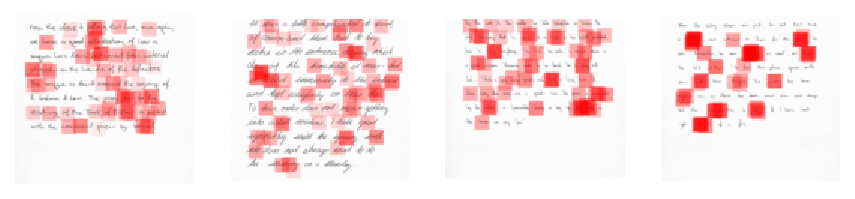
\includegraphics[width=\textwidth]{figures/fig_attention}
\caption{Attention weights (red, opacity proportional to weight) on four IAM validation pages.}
\label{fig:att}
\end{figure*}
}{}
\IfFileExists{sections/discussion.tex}{\section{Discussion}
\label{sec:discussion}
\textbf{What the evidence supports.}
A small student trained from scratch separates writers better than the foundation model it was distilled from, but the two corpora tell different stories.
IAM errors are low and optimistic: pages of one writer share scanner, pen and session, and a network with untrained features and adapted statistics already reaches 8.5\% on validation.
CVL, where all writers copy the same text, and Firemaker, where the scanner changes, are the better guides: 7.3\% EER on content-matched pairs and 3.3\% across corpora for ordinary writing.

\textbf{Disguise is the weak point.}
When the same writer changes style deliberately, EER rises to 24 to 32\%.
A verdict of ``likely forged'' therefore means ``unlike this writer's ordinary pages'', which a forger and a disguising writer can both produce.
We see this as a reason to keep the \emph{inconclusive} outcome and to collect more references written under varied conditions, not as a flaw to hide.

\textbf{More references help, but the evidence is thin.}
The gain from one to three references is visible on both corpora and in every seed, but the intervals overlap and the best fusion rule differed between corpora, so we advise using several references of the same writer and reporting all fusion rules until a separate validation set confirms one.

\textbf{Attention maps and synthetic pages.}
The deletion test does not support reading attention as an explanation (\Cref{sec:results}), and the font-rendered pages show only that fonts do not resemble real writers; neither measures learned imitation.
}{}
\IfFileExists{sections/limitations.tex}{\section{Limitations}
\label{sec:limits}
\textbf{No real impersonation data.}
Public corpora contain genuine pages by many writers but no pages in which one person copies another.
Our impostors are other writers, which is an easier case than a skilled forger; the content-matched CVL pairs make it harder but are still not imitations.
The reported error rates are therefore not forgery detection rates.

\textbf{Firemaker page 3 is disguise.}
The Firemaker authors ask writers to change their own style.
We use it only to measure how much scores move when the same writer writes differently, and we do not count it as forgery.

\textbf{Synthetic pages.}
The only synthetic pages we had are font-rendered text, not generated imitations of a particular writer.
We could not run a handwriting generator in the time available, so robustness to learned imitation is untested.

\textbf{Corpus effects.}
Pages of one IAM writer share a scanner, pen and session, so IAM error rates are optimistic; we therefore draw conclusions mainly from CVL and from Firemaker, which were never used for tuning.
We used a third-party copy of IAM.
All text is English, and most writers are adults who wrote under instruction, unlike exam answers written under time pressure.

\textbf{Scale.}
All models are small (a ResNet-18 trained on about 2,200 pages) and were trained on one laptop GPU; three seeds are reported, so confidence intervals are wide where few writers are available (for example five reference pages).
}{}
\IfFileExists{sections/conclusion.tex}{\section{Conclusion}
We built a page-level handwriting verifier that compares a questioned page with one or several reference pages and returns a calibrated score and a three-way verdict.
Trained from scratch on about 2,200 pages, it halves the error of frozen DINOv2 features (2.35\% EER on IAM, 7.30\% on CVL), transfers to a new corpus for ordinary writing (3.33\% on Firemaker), and gains from extra reference pages, but it is fooled by deliberate style change (24 to 32\% EER), and none of the training ingredients we ablated is demonstrated to help in a short schedule.
Because no public data show one person imitating another, our error rates are not forgery detection rates.

\textbf{Future work.}
The next steps are a real impersonation collection with volunteers, a handwriting generator to test learned imitation, multi-seed ablations at the full schedule, a validation set large enough to choose the fusion rule, and the four Indian languages for which data collection was paused.

\textbf{Reproducibility.}
Code, configurations, run logs, result files and the scripts that generate every table and figure are in the project repository; IAM, CVL and Firemaker are available from their owners under their own licences.

\textbf{AI-assistance disclosure.}
Claude (Anthropic) assisted with code, analysis scripts and drafting; the authors are responsible for the content.
The frozen DINOv2-small teacher is used during training only.
}{}

\appendices
\IfFileExists{sections/appendix.tex}{\section{Implementation details}
\label{app:impl}
\subsection{Preprocessing parameters}
Separator lines on IAM forms are found by a horizontal morphological opening with a 400~px kernel and a row-sum threshold of 30\% of the page width (retried with a 250~px kernel and 15\% for faint lines); the handwritten area lies between the second separator and the ``Name'' footer line, with a fallback to fixed fractions when a line is missing.
CVL pages use a 300~px kernel and a 20\% threshold for the line under the printed source text.
The background is estimated by a $25\times25$ morphological closing followed by a Gaussian blur of $\sigma=20$, and the page is divided by it.
A page is rejected when either side is shorter than 200~px or the aspect ratio exceeds 4, and as blank when the ink fraction (pixels darker than $0.75\times$ the median) is below $0.25\%$.
This threshold was lowered from $0.5\%$ after 34 CVL pages written with thin pens were wrongly marked blank.
Of the Kaggle real-versus-generated set, 2,352 pages were kept; duplicates and strip-shaped images were removed by the hash and geometry filters.

\subsection{Patch sampling}
Candidate windows are centred on a random subset of ink pixels (1,500 draws); a window is kept if its ink fraction reaches the first level of the sequence 5\%, 3\%, 1.5\%, 0.8\% at which at least $K$ windows qualify.
If even 0.8\% fails, windows with at least 0.4\% ink are resampled with replacement, and a page with none is rejected rather than padded.
For evaluation the random generator is seeded from a hash of the page path, so the same patches are used in every evaluation; the demonstration seeds it from a hash of the normalised image instead.

\subsection{Training procedure}
Training uses mixed precision, gradient clipping at 1.0, an exponential moving average of the weights (decay 0.999) for validation and testing, and validation every second epoch.
The training loop recovers from out-of-memory errors by halving the number of patches (down to 8), skips non-finite losses, and writes checkpoints safely on termination signals, so an interrupted run can resume; a resumed run refuses a checkpoint from a different seed.
Content-matched CVL batches pick two texts that enough writers have written and use only those writers; the nearest-neighbour batches use centroids recomputed every 10 epochs.
A label-shuffle control (writer labels permuted inside each batch) keeps the loss at $\ln 24=3.135$, confirming that no information leaks through page order or file names.

\subsection{Compute}
\begin{table}[t]
\caption{Measured compute on the RTX 4050 laptop GPU (6~GB).}
\label{tab:compute}
\centering\scriptsize
\begin{tabular}{ll}
\toprule
Item & Value \\
\midrule
GPU memory in training & about 3.5~GB \\
Time per epoch (70 steps, with distillation) & 25 to 28~s \\
Main run (three seeds) & about 50 min of training each \\
Ablation run (40 epochs) & about 20 min each \\
Reported runs in total & about 5 GPU hours \\
Demonstration inference & CPU only, about 2 to 3~s per comparison \\
\bottomrule
\end{tabular}
\end{table}

\section{Complete multi-reference results}
\label{app:multiref}
\Cref{tab:mrfull} gives every fusion rule at every number of references on the fixed writer sets used in \Cref{fig:multiref}, and \Cref{tab:mrn5} the smaller set of IAM writers with at least six pages that allows five references.
All entries are test EER (\%), mean $\pm$ standard deviation over three seeds; the sets use nested references and the same impostor queries for every $N$.
The maximum rule is lowest at $N=2$ on IAM and at $N=2,3$ on CVL, and the centroid is lowest at $N=3$ on IAM.
Differences between rules are of the order of the seed spread on IAM, so the choice of rule matters mainly on CVL.

\begin{table}[t]
\caption{Test EER (\%) for every fusion rule and number of references, on one fixed writer set per corpus.}
\label{tab:mrfull}
\centering\scriptsize
\setlength{\tabcolsep}{3pt}
\resizebox{\columnwidth}{!}{\begin{tabular}{llccc}
\toprule
Corpus (writers) & Rule & $N{=}1$ & $N{=}2$ & $N{=}3$ \\
\midrule
IAM (45) & mean & 2.25$\pm$0.05 & 1.79$\pm$0.19 & 1.59$\pm$0.21 \\
IAM (45) & max & 2.25$\pm$0.05 & 1.37$\pm$0.09 & 1.44$\pm$0.11 \\
IAM (45) & top-2 & 2.25$\pm$0.05 & 1.79$\pm$0.19 & 1.48$\pm$0.09 \\
IAM (45) & centroid & 2.25$\pm$0.05 & 1.57$\pm$0.11 & 1.22$\pm$0.12 \\
\midrule
CVL (62) & mean & 6.76$\pm$0.38 & 7.01$\pm$0.63 & 5.99$\pm$0.71 \\
CVL (62) & max & 6.76$\pm$0.38 & 4.68$\pm$0.44 & 3.31$\pm$0.20 \\
CVL (62) & top-2 & 6.76$\pm$0.38 & 7.01$\pm$0.63 & 5.13$\pm$0.18 \\
CVL (62) & centroid & 6.76$\pm$0.38 & 5.22$\pm$0.54 & 5.19$\pm$0.73 \\
\bottomrule
\end{tabular}
}
\end{table}

\begin{table}[t]
\caption{Test EER (\%) on the 17 IAM writers with at least six pages, which allows $N=5$.}
\label{tab:mrn5}
\centering\scriptsize
\setlength{\tabcolsep}{3pt}
\resizebox{\columnwidth}{!}{\begin{tabular}{lcccc}
\toprule
IAM, 17 writers with $\geq$6 pages & $N{=}1$ & $N{=}2$ & $N{=}3$ & $N{=}5$ \\
\midrule
mean & 1.99$\pm$0.32 & 1.42$\pm$0.33 & 1.18$\pm$0.06 & 0.93$\pm$0.23 \\
max & 1.99$\pm$0.32 & 1.13$\pm$0.03 & 1.18$\pm$0.10 & 1.13$\pm$0.33 \\
top-2 & 1.99$\pm$0.32 & 1.42$\pm$0.33 & 1.13$\pm$0.23 & 0.83$\pm$0.19 \\
centroid & 1.96$\pm$0.31 & 1.32$\pm$0.06 & 1.08$\pm$0.30 & 0.81$\pm$0.22 \\
\bottomrule
\end{tabular}
}
\end{table}

\section{Thresholds and calibration per seed}
\label{app:calib}
\Cref{tab:calib} lists, for each seed, the verdict thresholds fixed on validation trials (three references, centroid rule) and the expected calibration error of the raw score and of the two calibrators.
For IAM the two thresholds coincide because the corpus is separable on validation (\Cref{sec:results}).
Thresholds differ by up to 0.06 between seeds on CVL, so a deployed system would have to be calibrated for its own model and data.

\begin{table}[t]
\caption{Verdict thresholds (cosine) and expected calibration error per seed.}
\label{tab:calib}
\centering\scriptsize
\setlength{\tabcolsep}{2.5pt}
\resizebox{\columnwidth}{!}{\begin{tabular}{llccccc}
\toprule
Corpus & Seed & $\tau_{\mathrm{lo}}$ & $\tau_{\mathrm{hi}}$ & ECE raw & ECE Platt & ECE isotonic \\
\midrule
IAM & 0 & 0.888 & 0.888 & 0.213 & 0.066 & 0.010 \\
IAM & 1 & 0.884 & 0.884 & 0.218 & 0.066 & 0.009 \\
IAM & 2 & 0.898 & 0.898 & 0.222 & 0.078 & 0.008 \\
\midrule
CVL & 0 & 0.824 & 0.909 & 0.229 & 0.091 & 0.027 \\
CVL & 1 & 0.780 & 0.888 & 0.220 & 0.074 & 0.024 \\
CVL & 2 & 0.698 & 0.846 & 0.201 & 0.064 & 0.010 \\
\bottomrule
\end{tabular}
}
\end{table}

\section{Additional figures}
\label{app:figs}
\begin{figure}[t]
\centering
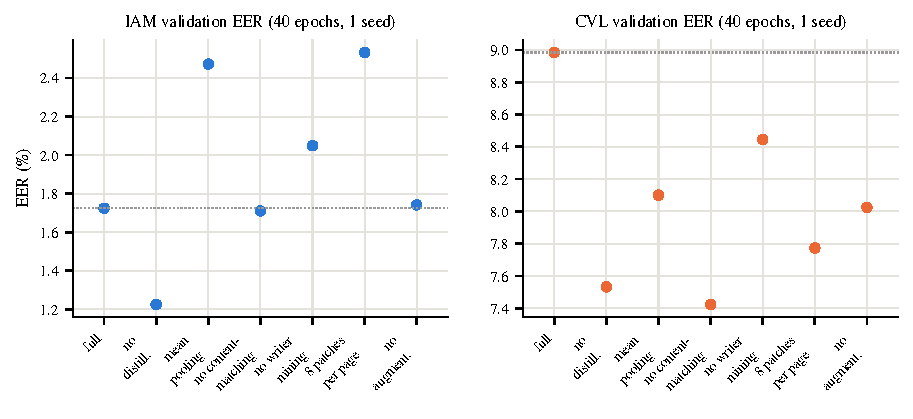
\includegraphics[width=\columnwidth]{figures/fig_ablation}
\caption{Validation EER of the ablation variants (40 epochs, one seed each); the dotted line is the full model.}
\label{fig:abl}
\end{figure}

\begin{figure}[t]
\centering
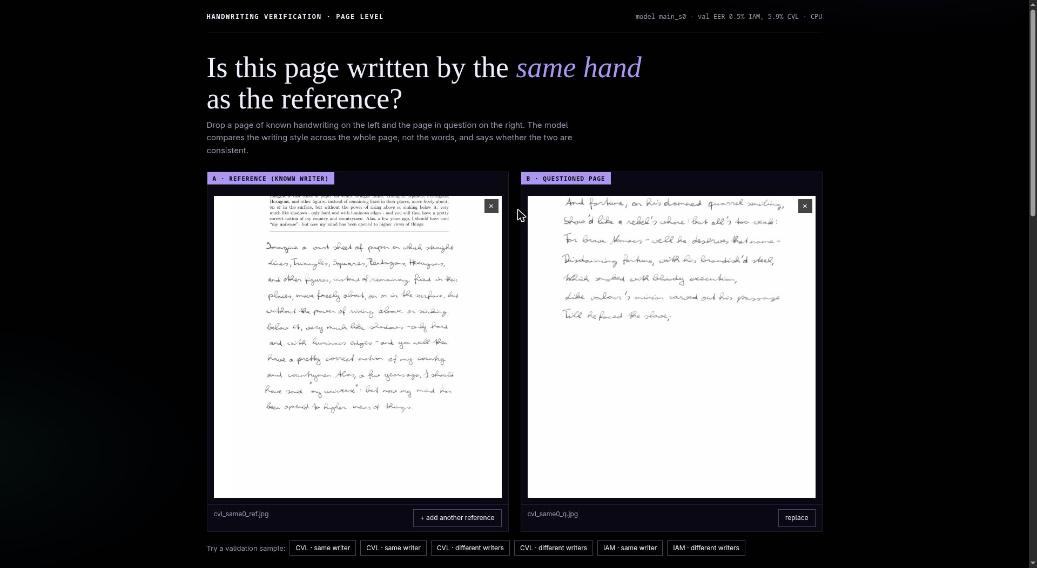
\includegraphics[width=\columnwidth]{figures/demo_inputs.jpg}
\caption{Demonstration service: the reference page and the questioned page are uploaded or chosen from validation samples.}
\label{fig:demo1}
\end{figure}

\begin{figure}[t]
\centering
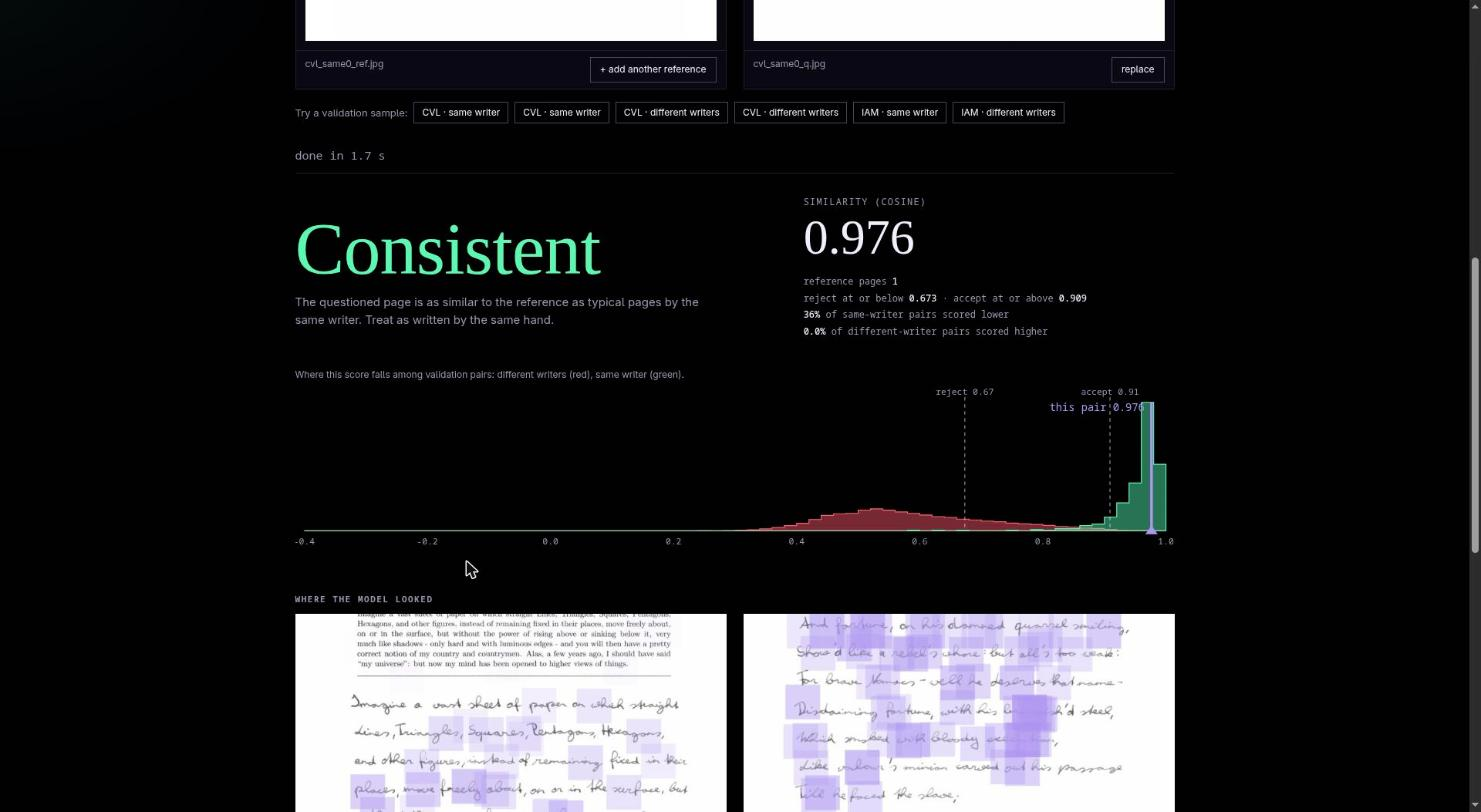
\includegraphics[width=\columnwidth]{figures/demo_result.jpg}
\caption{Demonstration result: verdict, similarity score, position of the score among validation pairs of different writers (red) and the same writer (green), and attention heatmaps.}
\label{fig:demo2}
\end{figure}

\section{Responsible use}
\label{app:ethics}
A verdict of \emph{likely forged} can damage a person, so the system is meant as decision support for a human examiner, not as evidence on its own.
Three properties make caution necessary.
First, the model measures similarity of writing style; a writer who changes style on purpose is rejected (\Cref{tab:fm}), and a skilled imitator has not been tested.
Second, the error rate at a strict operating point is high on content-matched pairs (\Cref{sec:results}), so a single page pair is weak evidence.
Third, thresholds are fitted on validation data of two corpora and may not hold for other paper, pens or scanners; phone photographs differ from the training scans.
The demonstration therefore prints these limits next to every result and returns \emph{inconclusive} when the score lies between the two thresholds.
All pages and models stay on the local machine; the demonstration does not store uploads.
Datasets were used under their own licences, and the IAM copy used here is third-party, so official registration is needed before the data are cited in a submission.

\section{Reproducibility checklist}
\label{app:repro}
\begin{table}[t]
\caption{Where each part of the study lives in the project repository.}
\label{tab:repo}
\centering\scriptsize
\setlength{\tabcolsep}{3pt}
\resizebox{\columnwidth}{!}{%
\begin{tabular}{ll}
\toprule
Part & Module \\
\midrule
Page cache, splits, leakage checks & \texttt{prep\_cache.py}, \texttt{manifests.py} \\
Patch sampler, content-matched batches & \texttt{data.py} \\
Encoder, losses & \texttt{model.py} \\
Training with resume and recovery & \texttt{train.py}, \texttt{run\_train.sh} \\
Baselines & \texttt{baselines.py} \\
Single-reference evaluation, Firemaker, synthetic pages & \texttt{eval.py} \\
Controlled multi-reference study & \texttt{multiref.py} \\
Verdict from saved scores & \texttt{verdict.py} \\
Attention maps and deletion test & \texttt{explain.py} \\
All tables, figures and the abstract & \texttt{report.py} \\
\bottomrule
\end{tabular}}
\end{table}
Each run stores its configuration, per-epoch log and result files; the three seeds are 0, 1 and 2, and all splits use seed 42.
The test sets and Firemaker were evaluated once per seed after training ended, and the two analysis errors found afterwards (overlapping verdict thresholds and a writer set that shrank with $N$) were corrected without retraining and are documented in the repository.
Every number in this paper is generated from the stored result files and listed with its source in a claim-to-evidence map, and the commands to repeat the experiments on GPU and CPU are in the repository documentation.
}{}

\printbibliography

\end{document}
